\cleardoublepage % memastikan bab baru dimulai di halaman ganjil (kanan)
\titlespacing{\chapter}{0pt}{-30pt}{5pt}
\chapter{ORGANISASI ATAU LINGKUNGAN KERJA PRAKTIK}
\label{chap:organisasi_lingkungan}
\titlespacing{\section}{0pt}{6pt}{6pt}
\section{Profil Perusahaan}
\label{sec:profil_perusahaan}
\begin{figure}[h]
    \centering
    
\includegraphics[width=0.45\textwidth]{images/Logo.png}
    \caption{Logo PT Nutech Integrasi}
    \label{fig:logo-nutech}
\end{figure}

PT Nutech Integrasi merupakan perusahaan yang bergerak di bidang teknologi informasi dan integrasi sistem sejak tahun 2006. Pada tahun 2017, PT Nutech Integrasi menjadi bagian dari Telkom Group melalui PT Multimedia Nusantara. Perusahaan ini memiliki visi menjadi mitra terpercaya dalam pengembangan ekosistem digital transportasi publik, dengan misi memberikan nilai tambah bagi pelanggan.
\section{Struktur Organisasi}
\label{sec:struktur_organisasi}
Struktur organisasi perusahaan terbentuk berdasarkan pembagian fungsi dan tanggung jawab untuk mendukung kegiatan operasional. Struktur ini dipimpin oleh \textit{President Director} yang didukung oleh \textit{Internal Audit Manager} dan \textit{BOD Secretary}, serta membawahi \textit{Director of Marketing \& Sales} dan \textit{Director of Finance, Risk \& Operation}. Pembagian struktur berfungsi untuk memastikan koordinasi berjalan secara efektif.

\textit{Director of Marketing \& Sales} membawahi fungsi pengembangan bisnis, pengembangan produk, dan pemasaran melalui \textit{General Manager Business \& Product Development}. Sementara itu, \textit{Director of Finance, Risk \& Operation} bertanggung jawab atas pengelolaan keuangan, manajemen risiko, operasional, serta fungsi pendukung perusahaan, termasuk \textit{Operation \& Delivery}. Setiap unit memiliki tanggung jawab sesuai bidangnya untuk mendukung pencapaian tujuan perusahaan. Struktur organisasi PT Nutech Integrasi secara keseluruhan ditunjukkan pada gambar:

\begin{figure}[ht]
    \centering
    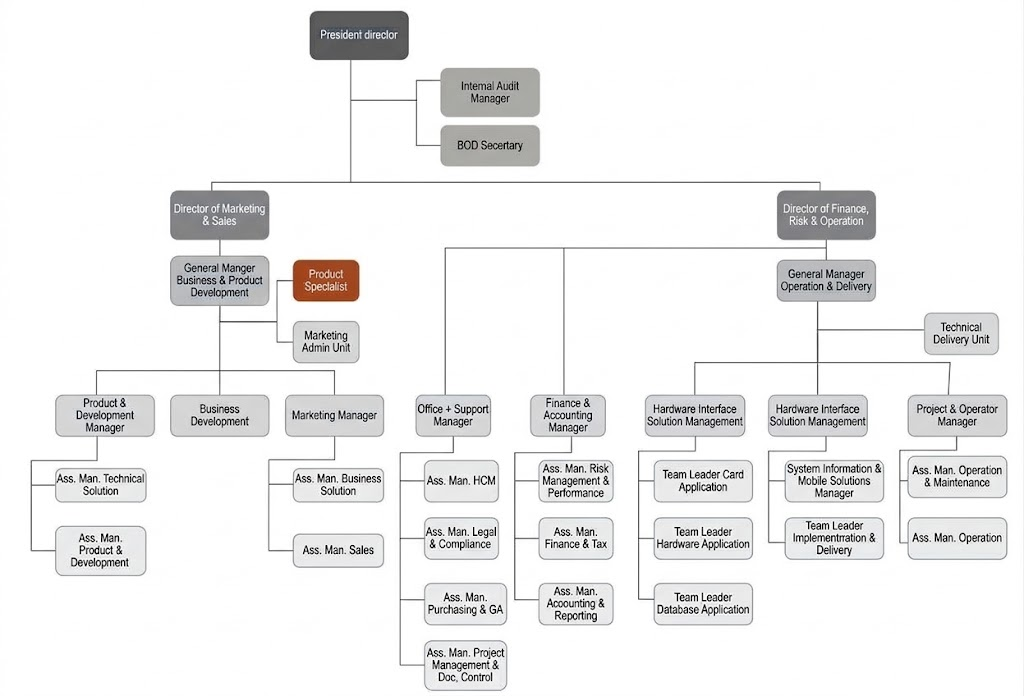
\includegraphics[width=0.9\textwidth]{images/organogram.jpg}
    \captionsetup{justification=centering}
    \caption{Struktur Organisasi PT Nutech Integrasi}
    \label{fig:struktur-organisasi}
\end{figure}

\section{Unit Kerja}
\label{sec:unit_kerja}
Penulis ditempatkan pada Divisi \textit{Business \& Product Development} dengan posisi sebagai \textit{Product Specialist}, sebagaimana ditandai dengan warna cokelat pada bagan struktur organisasi. Divisi ini bertanggung jawab dalam pengembangan bisnis dan perancangan solusi teknologi melalui analisis kebutuhan pelanggan, eksplorasi produk, serta penyusunan konsep \textit{Product Solution}. Kegiatan tersebut berkontribusi dalam mendukung pengembangan portofolio solusi dan identifikasi peluang bisnis perusahaan.

Selama pelaksanaan kerja praktik, pekerjaan penulis mencakup empat kegiatan utama, yaitu analisis proses bisnis, eksplorasi teknologi, perancangan solusi produk, serta penyusunan materi pendukung \textit{pre-sales}. Kegiatan tersebut diterapkan dalam kajian \textit{Smart Depot Management System}, pemetaan solusi \textit{Automatic Fare Collection} (AFC), serta eksplorasi peluang bisnis Penerangan Jalan Umum Tenaga Surya (PJUTS). Pembahasan lebih lanjut mengenai pelaksanaan dan hasil pekerjaan disajikan pada Bab III dan Bab IV.
\section{Lingkungan Kerja}
\label{sec:lingkungan_kerja}
Lingkungan kerja di PT Nutech Integrasi memiliki budaya kerja yang mendukung kolaborasi dan komunikasi antarunit. Selama pelaksanaan kerja praktik, kegiatan dilakukan melalui diskusi bersama tim, pembagian tugas, serta penyampaian hasil pekerjaan kepada pembimbing. Perusahaan juga menyediakan fasilitas pendukung berupa ruang kerja, akses internet, dan perangkat lunak yang digunakan untuk kegiatan analisis, dokumentasi, serta penyusunan materi \textit{Product Solution}.

Pelaksanaan kerja praktik di PT Nutech Integrasi menerapkan sistem kerja fleksibel, dengan sebagian besar kegiatan dilakukan secara \textit{Work From Office} (WFO) dan beberapa kegiatan secara \textit{Work From Anywhere} (WFA). Penulis beradaptasi dengan lingkungan profesional melalui koordinasi bersama tim, penyesuaian terhadap alur kerja divisi, serta penyelesaian tugas sesuai tanggung jawab yang diberikan. Pengalaman ini memberikan pemahaman mengenai pentingnya komunikasi, kerja sama, dan kemampuan beradaptasi dalam lingkungan kerja perusahaan.
